\chapter{Cycle 1: Understanding Unemployment in South Africa}
\begin{chapterintro}
In this chapter, we detail the findings of our first research cycle in which we focused on understanding the issues around unemployment. Section 5.1 is a discussion of the methodology we used in understanding unemployment in Cape Town South Africa, in section 5.2 we discuss our findings, in section 5.3 and 5.4 we discuss the implications of our findings and then we explain how we chose a design direction in section 5.5 and finally we conclude the chapter in section 5.6.
\end{chapterintro}

\section{Methods}

We conducted two student interviews, two trainer interviews and a workshop with the NGO, AT to better understand the problem from the views of our different participants. Similarly, we conducted a workshop, two student interviews and two trainer interviews with the other NGO, TZN. Both student and trainer participants were each given an informed consent form to sign after being informed of the purpose of the study.

The inputs from the trainers were collected to supplement the information to understand the unemployment issues faced by job seekers. The trainers served as intermediaries in the research and their inputs were supplementary to the job seekers’ inputs. The following paragraphs give details of the activities performed during Cycle 1.

Trainer interviews (2 per NGO): The job seeker’s trainers are first interviewed as intermediaries to provide entrant information about unemployed persons they coached and their understanding of unemployment itself.

In-depth Student Interviews (2 per NGO): The student job seekers’ interviews are then conducted to gain in-depth information from actual job seekers. We sought demographic information as well as information on the students’ previous jobs and training.

Brainstorming workshop (1 per NGO): The data collected was then triangulated by collecting information in an ideas generation workshop. Utilizing a workshop approach allowed us to obtain multiple views \cite{preece2002} in a single sitting. The first workshop session involved seven Co-designers (five unemployed or underemployed participants, the researcher, and research assistant).

Survey and Study Primer: First, the researcher asked a series of questions about the participants (nationality, mobile literacy and usage), and about struggles faced in job searching. Through this process, we identified problems together, triggering ideas that would be useful in the ideas brainstorming section of the workshop. Issues such as language barriers in speaking English and Afrikaans and lack of experience which were sought by employers were raised.

Ideas Brainstorm: Then a brainstorming section was undertaken, where each participant had a chance to suggest ideas or add to other ideas.

Prototyping session: Participants were given a chance to prototype their ideas after the discussion.

Ideas Presentation and discussion: The participants were then given a chance to discuss their ideas.

The researcher then selected a combination of ideas to tackle the issues raised. The selected idea was to develop a system that would gather participants’ personal information and would thereafter be used to market job opportunities for job seekers.

\section{Findings}

\subsection{Participants’ Demographics}

In Cycle 1 we interviewed four participants, two from each organisation. Table ~\ref{tab:job-seekers-interview-summary}  summarizes the employment-related information of our participants. Through the interviews, we found that our participants highest level of qualification ranged between grade 11, grade 12 and diplomas and had skills such as driving, waiting and cooking. We also found that the individuals had left their previous jobs because they did not earn enough, had no transport money to go the workplace, the work was too difficult, or they got a better job amongst other reasons. Two of the four participants had bank accounts whilst the other two did not. Although some of the participants could not speak English very well, they all gave themselves ratings of 3/5 to 5/5 in reading, speaking and writing English. They also rated themselves as being very employable with two rating themselves as 3/5 and another two giving themselves 5/5. Despite these, the participants admitted their shortcomings. Participant 4 stated: “those sites they need people with qualification which are high when I don't have”. Participant 1 stated: “as a security officer, sometimes I'm too busy with my job and I can't get information on time”. All four indicated that when they sought for jobs they did so through friends, and only one of them indicated he used his phone to find jobs. Three of our four participants did not only need jobs to look after themselves but had one or two children who depended on them.

All the participants had been employed before, with each one having had at least 3 different jobs in the past, the participants were still in search of new jobs. See Appendix A for the details of the findings. At the point of interview 3 of our 4 participants were jobless and the participant who had a job was seeking a better job by placing CVs where there are openings when he is not working.

\begin{table}[htbp]
\centering
\caption{Job seekers Interview Findings Summary}
\renewcommand{\arraystretch}{1.2}
\begin{tabularx}{\textwidth}{|X|>{\centering\arraybackslash}p{4cm}|}
\hline
\rowcolor{gray!30}
\textbf{Participants' Demographics} & \textbf{Number of Participants} \\
\hline

Highest qualification Matric or lower & 2/4 \\
\hline
Has a child or children to look after & 3/4 \\
\hline
Disabled & 0/4 \\
\hline
Had been employed before & 4/4 \\
\hline
Have bank accounts & 2/4 \\
\hline
Sought for jobs through friends & 4/4 \\
\hline
Sought for jobs using a mobile phone & 1/4 \\
\hline
Unemployed & 3/4 \\
\hline
Seeking for a job & 4/4 \\
\hline

\end{tabularx}
\label{tab:job-seekers-interview-summary}
\end{table}



%%%%%%%%%%%%%%%%%%%%%%%%%%%%%%%%%%%%%2
We conducted two workshops, one at TZN and the other at AT. For the workshops we had a different set of participants, however, the struggles indicated during the workshops were like those of the interviews. However, the workshop had an ideas generation section, and a prototyping section in addition to collecting information about the participants and their struggles. We found that most of the ideas suggested at the first workshop (at TZN), revolved around the creation of a job searching application. After ideas generation, the audience was to prototype their ideas as low-fidelity prototypes on little sticky notes, shown in Figure~\ref{fig:prototypes_ideas}. One of our five participants left the session before the prototyping time because of an obligation he had to attend to. Two of our remaining 4 job seekers stated that they could not prototype and left that to the other two outgoing participants to do. The two participants were very enthusiastic about a job searching application. The prototype of one of them was a logo for a job alert application and many of the prototypes were left to the researcher to create when the ideas came up. A divergent idea from the job finding app idea was the idea of a language learning app which could potentially tackle the lack of proficiency in English or Afrikaans.

\begin{figure}[h]
\centering
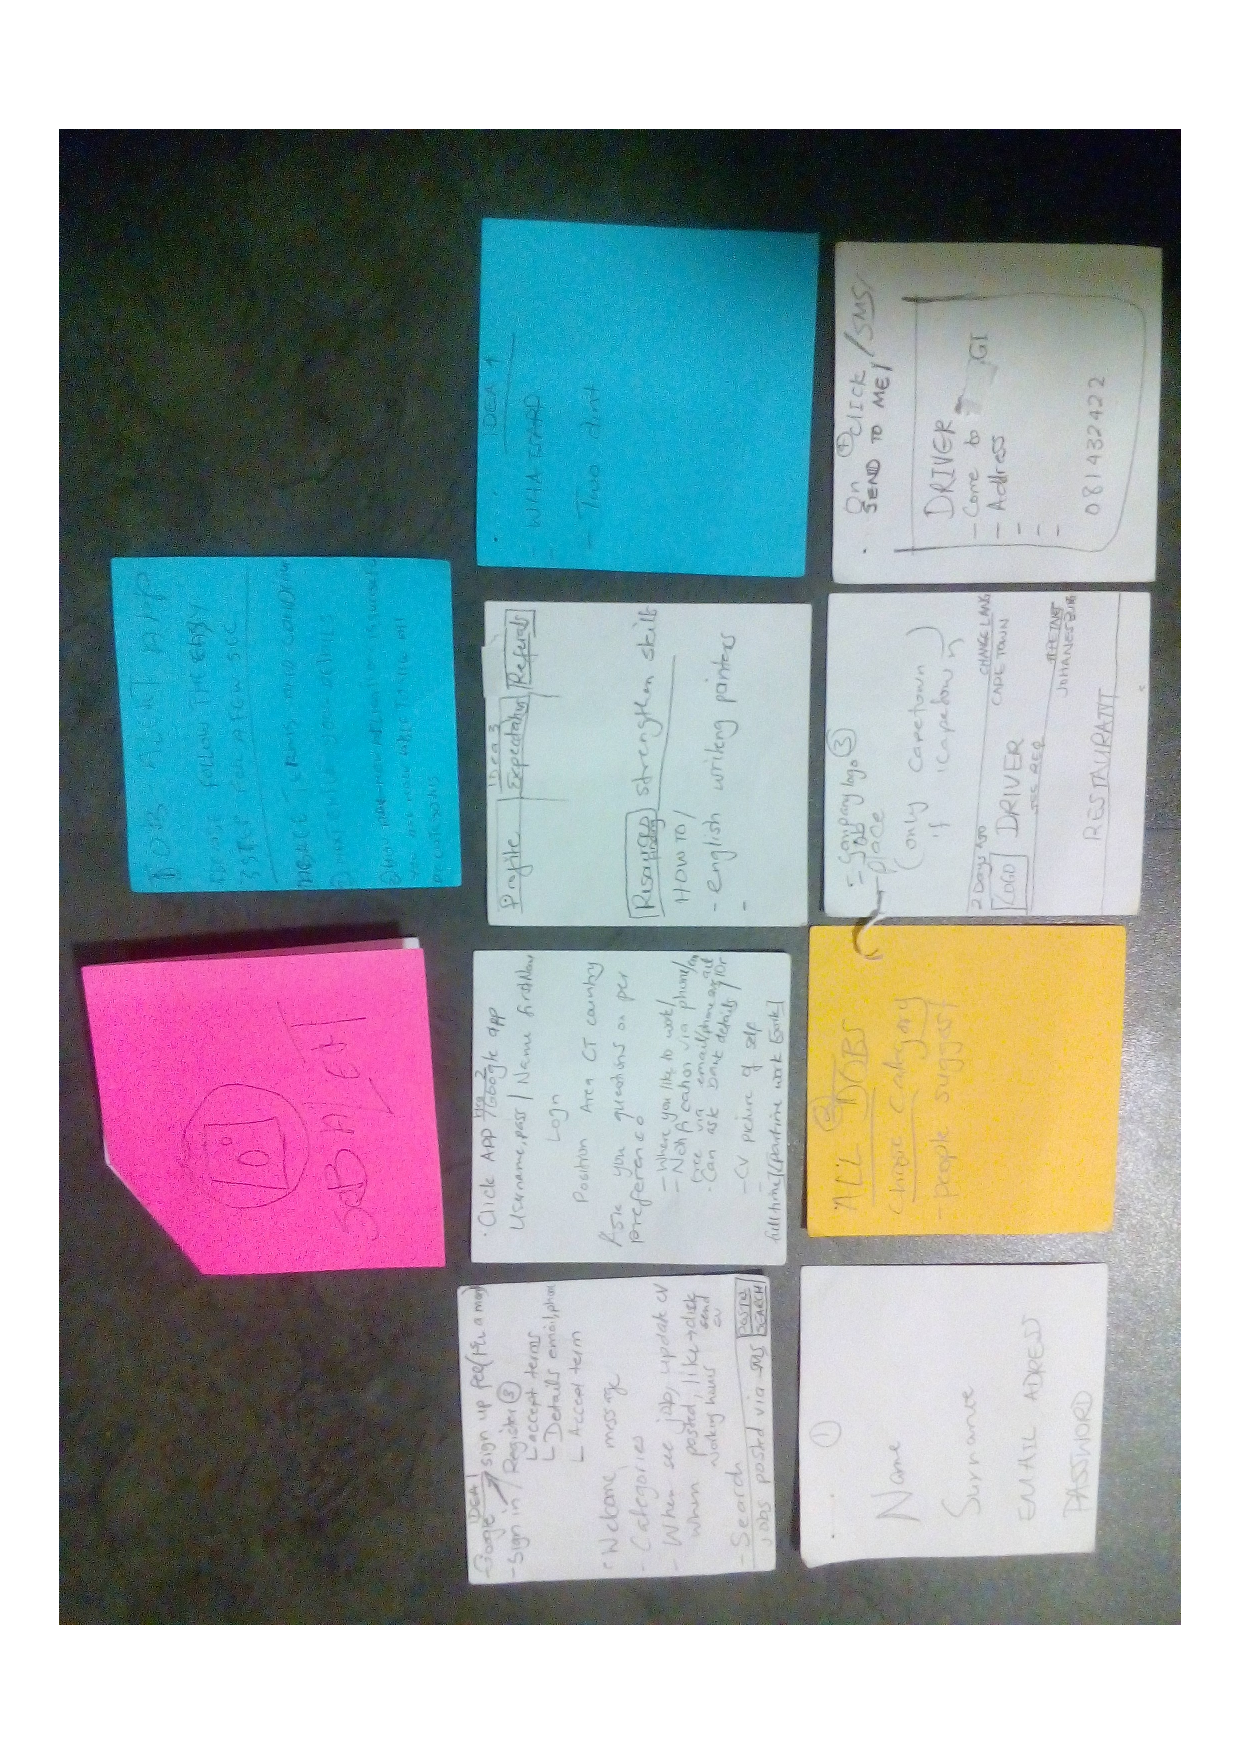
\includegraphics[angle=-90,width=0.9\linewidth]{figures/Figure 2: Prototypes of Ideas at Workshop 1.pdf}
\caption{Prototypes of Ideas at Workshop 1}
\label{fig:prototypes_ideas}
\end{figure}

Another workshop was then conducted at AT in Mfuleni, but it differed from the earlier workshop as the researcher allowed it to be largely driven by the trainers i.e. the intermediaries. Instead of a workshop with seven participants, we had a session with all the students that were present, graduates and a trainer of the JR class. The session included 34 students, seven graduates, a trainer and the researcher.

The focus of the second workshop was to discuss the struggles and some solutions for the unemployment problem as was also done in the workshop at Wynberg, however, this session yielded more issues. We found that working with a larger audience allowed u to collect richer data. The participants were free and were more open to explaining their struggles, they also had an opportunity to discuss amongst each other before suggestion solutions.

\subsection{Barriers to Employment}

Several issues were raised, some of which could be aided by a technological intervention.

Table ~\ref{tab:struggles_in_unemployment} and Table ~\ref{tab:potential_solutions_to_unemployment} below is an expansion of all the struggles and Proposed Solutions in Unemployment discussed in Co-design workshops with participants which can be broadly categorized as social conflict and hostility, shortage of funds, lack of information. We recognize the role of the trainers as intermediaries in directing the workshop, the intermediary assisted in getting the students to participate, facilitating the workshop by introducing it in a manner that made it appealing to the students, and it is possible that the session yielded more results because the students trusted the intermediary who took part in the Co-design session.

\begin{table}[htbp]
\centering
\caption{Struggles in Unemployment}
\renewcommand{\arraystretch}{1.2}
\begin{tabularx}{\textwidth}{|>{\centering\arraybackslash}p{0.8cm}|X|}
\hline
\rowcolor{gray!30}
\textbf{No.} & \textbf{Struggles in Unemployment or Job Searching} \\
\hline

\cellcolor{gray!15}\textbf{1} & Money to print and type CVs \\
\hline
\cellcolor{gray!15}\textbf{2} & Lack of experience to get jobs (freshman) \\
\hline
\cellcolor{gray!15}\textbf{3} & Lack of information about vacancies \\
\hline
\cellcolor{gray!15}\textbf{4} & Lack of qualification (freshman) \\
\hline
\cellcolor{gray!15}\textbf{5} & Lack of financial support \\
\hline
\cellcolor{gray!15}\textbf{6} & Concentration on Social Media \\
\hline
\cellcolor{gray!15}\textbf{7} & Language barrier (marketing barrier) \\
\hline
\cellcolor{gray!15}\textbf{8} & Lack of connections and references \\
\hline
\cellcolor{gray!15}\textbf{9} & Inability to market yourself \\
\hline
\cellcolor{gray!15}\textbf{10} & Bribery to get jobs \\
\hline
\cellcolor{gray!15}\textbf{11} & Social conflicts and enmity (get rid of your CV) \\
\hline
\cellcolor{gray!15}\textbf{12} & Employers requiring sexual encounter before giving a job \\
\hline
\cellcolor{gray!15}\textbf{13} & Lack of confidence \\
\hline
\cellcolor{gray!15}\textbf{14} & Lack of preparation for interviews \\
\hline
\cellcolor{gray!15}\textbf{15} & Lack of equipment \\
\hline
\cellcolor{gray!15}\textbf{16} & Laziness to look for jobs \\
\hline
\cellcolor{gray!15}\textbf{17} & Short employment duration (working knowing the contract will end) \\
\hline
\cellcolor{gray!15}\textbf{18} & Not enough jobs \\
\hline
\end{tabularx}
\label{tab:struggles_in_unemployment}
\end{table}

\begin{table}[htbp]
\centering
\caption{Potential Solutions to Unemployment}
\renewcommand{\arraystretch}{1.2}
\begin{tabularx}{\textwidth}{|>{\centering\arraybackslash}p{0.8cm}|X|}
\hline
\rowcolor{gray!30}
\textbf{No.} & \textbf{Suggested Solutions to the Job Searching Problems} \\
\hline

\cellcolor{gray!15}\textbf{1} & Be active in the community \\
\hline
\cellcolor{gray!15}\textbf{2} & Do volunteer work \\
\hline
\cellcolor{gray!15}\textbf{3} & Print out information to public places \\
\hline
\cellcolor{gray!15}\textbf{4} & Investing in one’s self \\
\hline
\cellcolor{gray!15}\textbf{5} & A partnership between college and companies (allowing students to gain experience early) \\
\hline
\cellcolor{gray!15}\textbf{6} & Stop depending on someone (partner) \\
\hline
\cellcolor{gray!15}\textbf{7} & Government and the community to create jobs \\
\hline
\cellcolor{gray!15}\textbf{8} & Companies should allow online application \\
\hline
\cellcolor{gray!15}\textbf{9} & Let secondary school students know not to go to university but college \\
\hline
\cellcolor{gray!15}\textbf{10} & Meet and discuss jobs once a week \\
\hline
\cellcolor{gray!15}\textbf{11} & The government can provide skills \\
\hline
\cellcolor{gray!15}\textbf{12} & People with high qualification to come and give motivational speeches \\
\hline

\end{tabularx}
\label{tab:potential_solutions_to_unemployment}
\end{table}

Although many of the barriers identified (listed in Table ~\ref{tab:struggles_in_unemployment}), in our first cycle were not direct ICT problems some could be aided with an improved ICT architecture for the target audience. It is apparent that, by not attending to improving technologies for disadvantaged communities, the digital gap between the rich and poor becomes wider and wider \cite{heeks2008}. However, there are unknown side-effects that may arise from leaping using some form of pre-existent technology \cite{elkhatib2015}, thus, the appropriation of the technology is needful \cite{david2013} and was achieved by co-designing with potential end-users.


%%%%%%%%%%%%%%%%%%%%%%%%%%%%%%%%%%%%%%%%%%%%%%%%%%%%%% 3


\begin{table}[htbp]
\centering
\caption{Potential ICT Enablers (Part 1)}
\label{tab:ict_enablers_part1}
\renewcommand{\arraystretch}{1.2}
\begin{tabularx}{\textwidth}{|>{\centering\arraybackslash}p{0.8cm}|p{2.2cm}|X|X|X|}
\hline
\rowcolor{gray!30}
\textbf{No.} & \textbf{Idea Name} & \textbf{Purpose} & \textbf{Problem tackled / Opportunity} & \textbf{Feasibility and Implementation Challenge} \\
\hline

\cellcolor{gray!15}\textbf{1} & Fund Finder & Find funding for individuals to further their education and become more employable. & Job seekers willing to further their studies. & Requires having the means to post different scholarships frequently. Funders would need the motivation to post on the application. \\
\hline

\cellcolor{gray!15}\textbf{2} & Problem Assessment App & Determine the major cause of joblessness and direct everyone appropriately. & Struggles vary & Human needed \\
\hline

\cellcolor{gray!15}\textbf{3} & Digital Jobs Notice Board (Public) & Provide information about jobs which job seekers scarcely get due to lack of devices, connectivity or little knowledge on searching for jobs online. & Lack of information; Lack of search skills & Digital notice-board needs to be managed to post relevant information and are expensive. General vacancies \\
\hline

\cellcolor{gray!15}\textbf{4} & Digital Jobs Notice Board (Mobile) & Provide information about jobs which job seekers scarcely get due to lack of devices, persistent connectivity or little knowledge on searching for jobs online. & Job seekers lack information about available vacancies or opportunities; Job seekers lack high-level technical skills to search for jobs online. & Requires smartphones and some connectivity to update the jobs list. Can be used while performing other tasks. Can be personalized for the owner of the device to see more relevant results. \\
\hline

\end{tabularx}
\end{table}


%%%%%%%%%%%%%%
\begin{table}[htbp]
\centering
\caption{Potential ICT Enablers (Part 2)}
\label{tab:ict_enablers_part2}
\renewcommand{\arraystretch}{1.2}
\begin{tabularx}{\textwidth}{|>{\centering\arraybackslash}p{0.8cm}|p{2.2cm}|X|X|X|}
\hline
\rowcolor{gray!30}
\textbf{No.} & \textbf{Idea Name} & \textbf{Purpose} & \textbf{Problem tackled / Opportunity} & \textbf{Feasibility and Implementation Challenge} \\
\hline

\cellcolor{gray!15}\textbf{5} & Talent Registry & Register your qualification, expertise and experience to get offers. & Skills marketing platform & Requires a means to be continually adding job seekers to the system with little or no effort from job seekers. Requires motivation for employers to continually search for job seekers online through the application. \\
\hline

\cellcolor{gray!15}\textbf{6} & Job Searching App & Find available jobs in different sectors in a manner suited to low-income earning job seekers. & Means to find jobs and apply directly & Many existing applications; Existing applications do not sooth low-skilled individuals well \\
\hline

\cellcolor{gray!15}\textbf{7} & Language Learning App & Learn a language of communication required for a job. & Learn a language for a job & Content must be deep but presented in a way that it is easy to learn \\
\hline

\end{tabularx}
\end{table}
%%%%%%%%%%%%%%%%%%%%%%%%%%%%%%%%%%%%%%%%%%%%%%%%%%%%%%%%%%%%%%%%%%%%%%%%%%%%%%%

In the following paragraphs, we discuss the different potential IT directions in Table ~\ref{tab:ict_enablers_part1} and Table ~\ref{tab:ict_enablers_part2}, the opportunities and the challenges associated with their implementation.

\subsubsection*{Idea One: Fund Finder}

Individuals do not have money or funding to study but are willing to further their studies. All the participants we interviewed in cycle one, were willing to further their studies. However, implementing this requires having the means to post different scholarships/bursaries/ loans to the app frequently. Secondly, funders would need the motivation to post on the application.

This idea can be linked with idea number five: Talent Registry, to ensure that funders can view the profiles of the individuals they would like to fund to know what talents they have. For this research, our goal was to identify a research direction, that is an issue amid the issues and design an architecture or artefact that will be tested to address the issue zoomed on.

\subsubsection*{Idea Two: Problem Assessment App}

Job seekers face different difficulties, this would require the application to understand each job seeker and thereafter guide him/her appropriately. However, this requires human expert/s to handle cases that have not been pre-coded. Secondly, there are many different directions to guide job seekers because of the great variation in struggles, elicited in Table \ref{tab:struggles_in_unemployment}, as such an AI system would have to be well trained to be effective.

\subsubsection*{Idea Three: Digital Jobs Notice Board (Public)}

Having a public display where job seekers can find information on available jobs can be useful because job seekers lack information about available vacancies or opportunities. They also lack high-level technical skills to search for jobs online, so a centrally operated jobs notice board can assist job seekers to find jobs. However, it may be very expensive to purchase a sizable digital notice board. The displayed offers must be generic for its multiple viewers and not suited to a specific need.

\subsubsection*{Idea Four: Digital Jobs Notice Board (Mobile)}

A notice board can also be developed as a mobile application. When a notice board is developed as a mobile application there is an opportunity to personalize the notice board for the device owner, for example in terms of job types or location to search for jobs. To create an application as a notice board, the application would have to be designed to need little or no input from the user, to mediate the need for operational skills. However, this requires the job seeker to own a smartphone and have connectivity to update the jobs list. Such an application has an advantage that the user can use it while performing other tasks.

\subsubsection*{Idea Five: Talent Registry}

Another idea is to create a platform where job seekers can market their skills online to potential employers. This will require that the job seekers are added to a growing, well-monitored database continually. Secondly, it requires employers to continually search for job seekers online through the application.

\subsubsection*{Idea Six: Job Searching App}

There are many job-finding websites, however, they are not well suited for low-skilled workers. A new application created for the same purpose would have to be differentiated. A new application can be designed to provide a mean for low-income, low-skilled individuals to find jobs and apply easily.

\subsubsection*{Idea Seven: Language Learning App}

An application can be developed to allow non-Afrikaans natives or non-English natives to learn a language/s that may be required to apply for certain vacancies. However, mastering a language can take a long time and job seekers may not be willing to put hours into learning a new language. Some already indicated they could not take part in the Co-design sessions because of job seeking, part-time jobs or children they had to attend to.

The ideas that have emerged from the entire cycle one can be grouped in the following technological categories:

\begin{enumerate}
\item Information and knowledge dissemination technology on how and where to seek employment

\item Application to find jobs in a simple way unlike CareerJet and other websites

\item Professional networking site like LinkedIn but oriented to low-skilled individuals  

\item Applications to teach job seekers English and Afrikaans to improve employability
\end{enumerate}

%%%%%%%%%%%%%%%%%%%%%%%%%%%%%%%%%%%%%%%%%%%%%%%%%%%%%%% 4
\section{Discussion: Implications for the Methodology}

By performing a combination of activities and methods of collecting data, we learnt that the tools and techniques designed for a Co-design project must be flexible so that it can be adapted to fit users’ contexts. We learnt that workshops work well when collecting information that is not personal but common for a group, to allow individuals to discuss without feeling cornered whereas, it is important to have one-on-one sessions when one needs inputs on preferences and experiences of individual participants. Thus, we had to trade-off using workshops for consensual information collection and one-on-one sessions for in-depth discussions and preferential views. 

We also learnt that workshops are not ideal for prototyping with low-skilled participants as some participants may not be comfortable expressing themselves through drawing or writing. In our case, some participants left the prototyping activity to others. This indicates the importance of having alternative prototyping approaches that are inclusive of participants with varying levels of confidence and skill. 

Working with intermediaries (trainers) proved to be beneficial as they facilitated engagement and helped participants feel more comfortable contributing. However, their involvement may also influence the type of responses obtained. This highlights the need to balance facilitator involvement to ensure that participants’ voices remain authentic.

\section{Discussion: Implications for Design for Unemployment}
\label{sec:implications_design_unemployment}
From the findings, it is evident that unemployment is not caused by a single factor but rather a combination of social, economic and informational challenges. Therefore, any ICT intervention must be designed to address multiple challenges simultaneously or focus on a key leverage point.

The lack of access to timely and relevant job information suggests that systems should prioritise information dissemination. However, simply providing information is not sufficient; the information must be accessible, understandable and actionable for low-skilled users.

The preference for using friends and social networks to find jobs indicates that trust plays a crucial role in job searching. ICT solutions should therefore incorporate social elements or leverage existing trusted networks.

Additionally, the limitations in digital literacy and access to devices suggest that systems should be simple, require minimal interaction and be usable on low-end devices. Designing for intermittent connectivity and low data usage is also essential.


%======================================
\section{Considerations for Idea Selection}
In Cycle 1, we evaluated potential intervention directions based on four primary considerations: resource constraints, project timeline, job-seeker priorities, and NGO institutional interests.

\begin{itemize}
\item \textbf{Research Resources:} Given our limited budget, we could not procure the specialized equipment required to implement several of the proposed ideas identified in Table~\ref{tab:ict_enablers_part1} and Table~\ref{tab:ict_enablers_part2}.
\item \textbf{Time-bound Feasibility:} The research required completion within a two-year period, a timeframe that also had to accommodate participant recruitment, data collection, and analysis. To reduce the time spent on recruitment, we partnered with NGOs to gain access to co-located groups of job seekers rather than seeking participants individually.
\item \textbf{Job-seeker Priorities:} We prioritized interventions addressing the participants’ most urgent needs. Although participants suggested both language learning and job-searching applications, we observed that job seekers already spent significant time on platforms like Indeed, Giraffe, and Gumtree. This observation "enacted" our focus on job searching, a deliberate methodological move within our Tell-Make-Enact cycle. Given that approximately 50\% of participants lacked smartphones or stable connectivity, we developed a web-based platform (mobisite) that utilized free internet access at NGO venues while remaining accessible via personal mobile devices. As discussed in Section~\ref{sec:implications_design_unemployment}, designs must accommodate the users’ available skills and digital proficiency, and while upskilling is valuable, our participants' immediate priority was securing income to support their dependents.
\item \textbf{NGO Institutional Interests:} We aligned our research with the objectives of our partner NGOs. TZN required support for student CV editing and interview preparation, while AT sought insights into the effectiveness of their Job Readiness (JR) program. Because sourcing human volunteers for CV assistance was not always feasible or consistent, automating CV creation provided a sustainable solution for both partners.
\end{itemize}

Based on these considerations, we evaluated the generated ideas for further development. Concepts such as the Fund Finder and Talent Registry were deemed difficult to sustain due to their reliance on continuous input from external stakeholders. Similarly, the Problem Assessment App was found too complex to implement due to its requirement for advanced intelligence and human intervention. While public digital notice boards offered utility, they were prohibitively costly and lacked personalization, and language learning applications required a time investment that did not align with the participants' immediate need for employment.

Ultimately, the Digital Jobs Notice Board (Mobile) and Job Searching App emerged as the most feasible and impactful solutions. These ideas directly address the lack of information and can be tailored to suit the needs of low-skilled users. Consequently, we selected the final direction of developing a mobile-based job searching solution that simplifies access to job information and reduces the effort required to find and apply for work.

\section{Conclusion}

In Cycle 1, we developed a comprehensive understanding of the challenges faced by unemployed individuals in South Africa. Through interviews and workshops, we identified key barriers such as a lack of information, financial constraints, and limited access to technology.

In applying these methods, we learned that the tools and techniques designed for a Co-design project must be flexible to adapt to the users' specific contexts. We found that workshops work well when collecting information that is common for a group, as this allows individuals to discuss without feeling cornered. Conversely, one-on-one sessions are important when we need inputs on the preferences and experiences of individual participants. Thus, we had to trade-off using workshops for group information collection and one-on-one sessions for in-depth discussions.

Although the participants made several contributions during ideas generation, we found that ideas selection could not be highly Co-designed because our participants had different views. We interacted with them at different sessions, and they were not available to meet in one place at the same time. At the heart of many of our participants was an urgent need to earn money to sustain their own living expenses and those of their dependents. Yet despite this urgency, individuals did not get jobs because they had limited online job searching knowledge among other obstacles that hindered them from getting jobs.

By synthesizing these findings, we identified that a mobile-based job searching solution was the most impactful and feasible direction for development in subsequent cycles. The findings highlighted the importance of designing technology solutions that are accessible, simple, and relevant to the target users.
%******************************************